% \documentclass[aspectratio=169,notes]{beamer}
\documentclass[aspectratio=169]{beamer}
\usetheme[faculty=phil]{fibeamer}
\usepackage{polyglossia}
\setmainlanguage{english} %% main locale instead of `english`, you
%% can typeset the presentation in either Czech or Slovak,
%% respectively.
\setotherlanguages{russian} %% The additional keys allow
%%
%%   \begin{otherlanguage}{czech}   ... \end{otherlanguage}
%%   \begin{otherlanguage}{slovak}  ... \end{otherlanguage}
%%
%% These macros specify information about the presentation
\title[Theoretical Mechanics]{Theoretical Mechanics, Lab 7: STATICS 2} %% that will be typeset on the
\subtitle{Statics: multiple bodies
\\ \ \\ \ 
         } %% title page.
\author{Oleg Bulichev}
%% These additional packages are used within the document:
\usepackage{ragged2e}  % `\justifying` text
\usepackage{booktabs}  % Tables
\usepackage{tabularx}
\usepackage{tikz}      % Diagrams
\usetikzlibrary{calc, shapes, backgrounds}
\usepackage{amsmath, amssymb}
\usepackage{url}       % `\url`s
\usepackage{listings}  % Code listings
% \usepackage{subfigure}
\usepackage{floatrow}
\usepackage{subcaption}
\usepackage{mathtools}
\usepackage{todonotes}
\usepackage{fontspec}
\usepackage{multicol}
\usepackage{pdfpages}
\usepackage{wrapfig}
\usepackage{animate}
\usepackage{booktabs}
\usepackage{multirow}
% \usepackage{graphicx}
\usepackage{colortbl}

\graphicspath{{resources/}}
\frenchspacing

\setbeamertemplate{caption}[numbered]
\usetikzlibrary{graphs}

% \usepackage[backend=biber,style=ieee,autocite=footnote]{biblatex}
% \addbibresource{biblio.bib}
% \DefineBibliographyStrings{english}{%
%   bibliography = {References},}

\newcommand{\oleg}[2][] {\todo[color=red, #1] {OLEG:\\ #2}}
\newcommand{\fbckg}[1]{\usebackgroundtemplate{\includegraphics[width=\paperwidth]{#1}}}%frame background

\usepackage[framemethod=TikZ]{mdframed}
\newcommand{\dbox}[1]{
\begin{mdframed}[roundcorner=3pt, backgroundcolor=yellow, linewidth=0]
\vspace{1mm}
{#1}
\vspace{1mm}
\end{mdframed}
}

\begin{document}
\setlength{\abovedisplayskip}{0pt}
\setlength{\belowdisplayskip}{0pt}
\setlength{\abovedisplayshortskip}{0pt}
\setlength{\belowdisplayshortskip}{0pt}

\fbckg{fibeamer/figs/title_page.png}
\frame[c]{\setcounter{framenumber}{0}
    \usebeamerfont{title}%
    \usebeamercolor[fg]{title}%
    \begin{minipage}[b][6.5\baselineskip][b]{\textwidth}%
        \textcolor{black}{\raggedright\inserttitle}
    \end{minipage}
    % \vskip-1.5\baselineskip

    \usebeamerfont{subtitle}%
    \usebeamercolor[fg]{framesubtitle}%
    \begin{minipage}[b][3\baselineskip][b]{\textwidth}
        \raggedright%
        \insertsubtitle%
    \end{minipage}
    \vskip.25\baselineskip
}
%   \frame[c]{\maketitle}

\fbckg{fibeamer/figs/common.png}


\section*{Tasks}

\begin{frame}[t]{Task 1 (mine)}
    \framesubtitle{}
    \begin{columns}[T,onlytextwidth]
        \begin{column}{0.49\textwidth}
            Find reaction forces in supports of the construction systems. The size of all objects and the loads are given.
        \end{column}
        \begin{column}{0.49\textwidth}
            \begin{figure}[H]
                \centering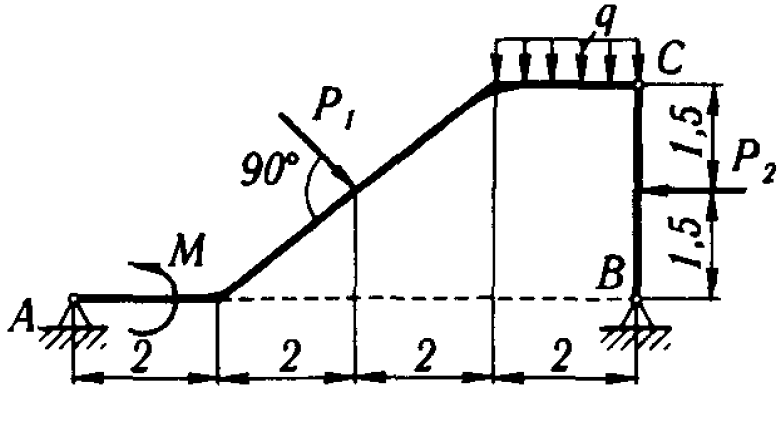
\includegraphics[height=6cm,width=1\textwidth,keepaspectratio]{image23.png}
            \end{figure}
        \end{column}
    \end{columns}
    \end{frame}

    \begin{frame}[t]{Task 2 (yours): solve "б", using ideal beam as 2nd body}
        \framesubtitle{}
        \begin{columns}[T,onlytextwidth]
            \begin{column}{0.49\textwidth}
                Find reaction forces in supports of the construction systems. The size of all objects and the loads are given.
            \end{column}
            \begin{column}{0.49\textwidth}
                \begin{figure}[H]
                    \centering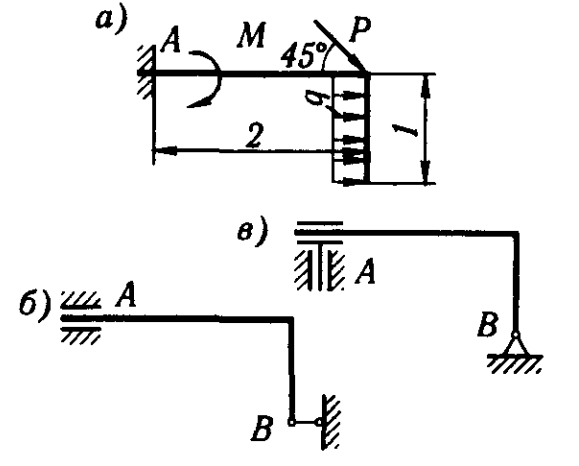
\includegraphics[height=6cm,width=1\textwidth,keepaspectratio]{image21.png}
                \end{figure}
            \end{column}
        \end{columns}
        \end{frame}

\begin{frame}[t]{Task 3 (yours): \href{https://easy-physic.ru/statika-podgotovka-k-olimpiadam/}{solution (rus)}, \href{https://colab.research.google.com/drive/1P1pg1yDU34CCFsNo2hBpK78VtTmlch8r?usp=sharing}{Collab}
            }
        \framesubtitle{}
        \begin{columns}[T,onlytextwidth]
            \begin{column}{0.49\textwidth}
                A bar with a weight of $m$ and two identical weights of $2m$ each with light threads are attached to two blocks. The system is in equilibrium. There is no friction in the axes of the blocks. Each "block" on a beam is equal to $l$.
                \medskip

                Determine the string tension forces and the forces with which the stand acts on the weights $T$.
            \end{column}
            \begin{column}{0.49\textwidth}
                \begin{figure}[H]
                    \centering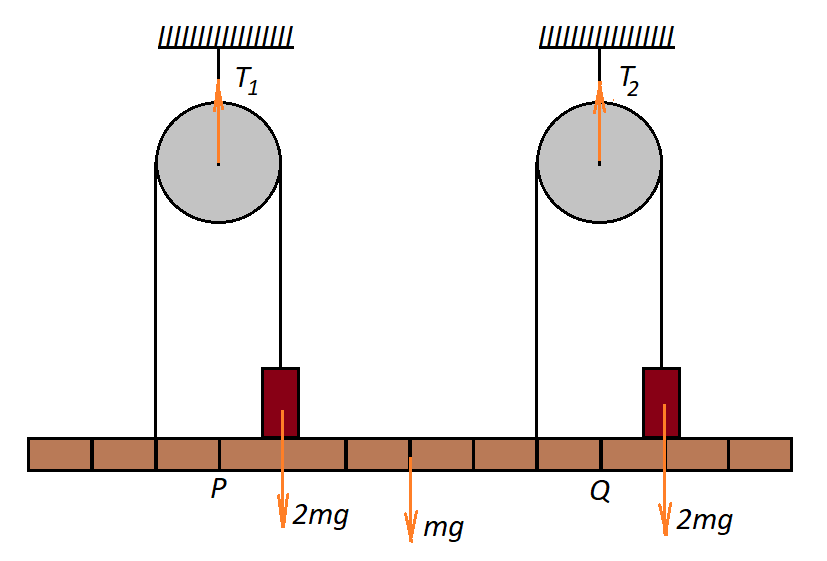
\includegraphics[height=6cm,width=1\textwidth,keepaspectratio]{image12.png}
                    \label{fig:image12}
                \end{figure}
            \end{column}
        \end{columns}
        \end{frame}

\section*{Expand your horizon}

\begin{frame}[t]{Disney research}
    \framesubtitle{Video}
    \vspace*{-0.6cm}
        \begin{figure}[H]
            \href{http://www.youtube.com/watch?v=DfznnKUwywQ}{
                \centering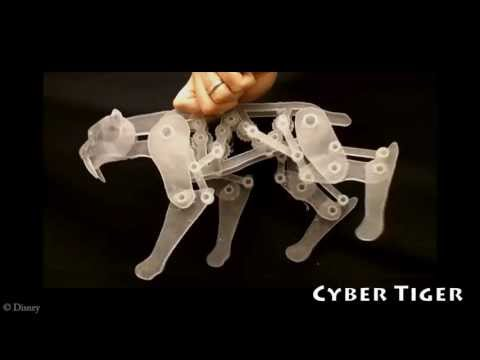
\includegraphics[height=6cm,keepaspectratio]{image14.jpg}}
        \end{figure}
    \end{frame}

\section*{Tasks (continue)}

\begin{frame}[t]{Task 4 (yours): M (rus) 4.49
    }
\framesubtitle{}
    \begin{figure}[H]
        \begin{subfigure}{0.69\textwidth}
            \centering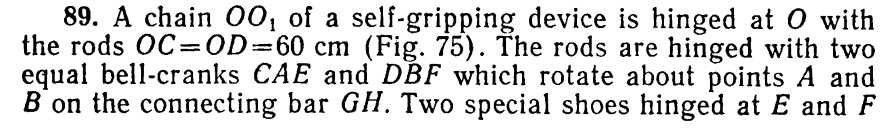
\includegraphics[height=6cm,width=1\textwidth,keepaspectratio]{image19.png}
            \label{fig:image19}
            \centering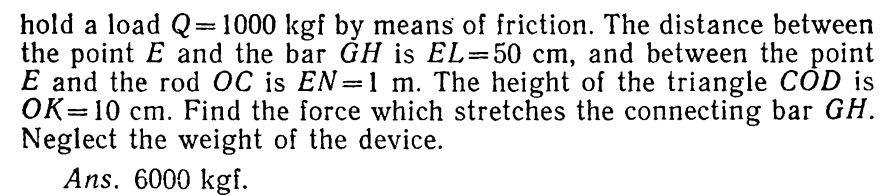
\includegraphics[height=6cm,width=1\textwidth,keepaspectratio]{image18.png}
            \label{fig:image18}
        \end{subfigure}
        \begin{subfigure}{0.29\textwidth}
            \centering
\includegraphics[height=6cm,width=1\textwidth,keepaspectratio]{image20.png}
            \label{fig:image20}
        \end{subfigure}
    
    \label{fig:}
    \end{figure}
\end{frame}

\fbckg{fibeamer/figs/last_page.png}
\frame[plain]{}
\end{document}